\documentclass{article}
\usepackage{graphicx}
\usepackage{caption}

\title{BOTNET vs CLOUD INFRASTRUCTURE}
\author{Nicolò Vinci  \\
	\and 
	Marcello Meschini \\
	}
 
\date{May 4, 2021}

\begin{document}

\maketitle

\section{Introduction}
\label{intro}

\subsection{Mandatory fields}
\label{mfields}

\begin{itemize}
\item Course: Fog and Cloud Computing 2021
\item Architecture: Botnet vs Cloud Infrastructure
\item Group number: 11
\item Authors:

\begin{itemize}
\item[-] Marcello Meschini marcello.meschini@studenti.unitn.it
\item[-] Nicolò Vinci nicolo.vinci@studenti.unitn.it
\end{itemize}

\end{itemize}

\section{Project idea} 
\label{idea}
Our idea is to create a scenario where a botnet mounts a DDoS attack against a server running on a PaaS infrastructure. The main objective is to understand and show how cloud technologies allow to absorb such an attack and handle sudden traffic increases. 
To implement this scenario we plan to create the botnet in the IaaS infrastructure and a server running a simple web application in the PaaS infrastructure.

\begin{center}
	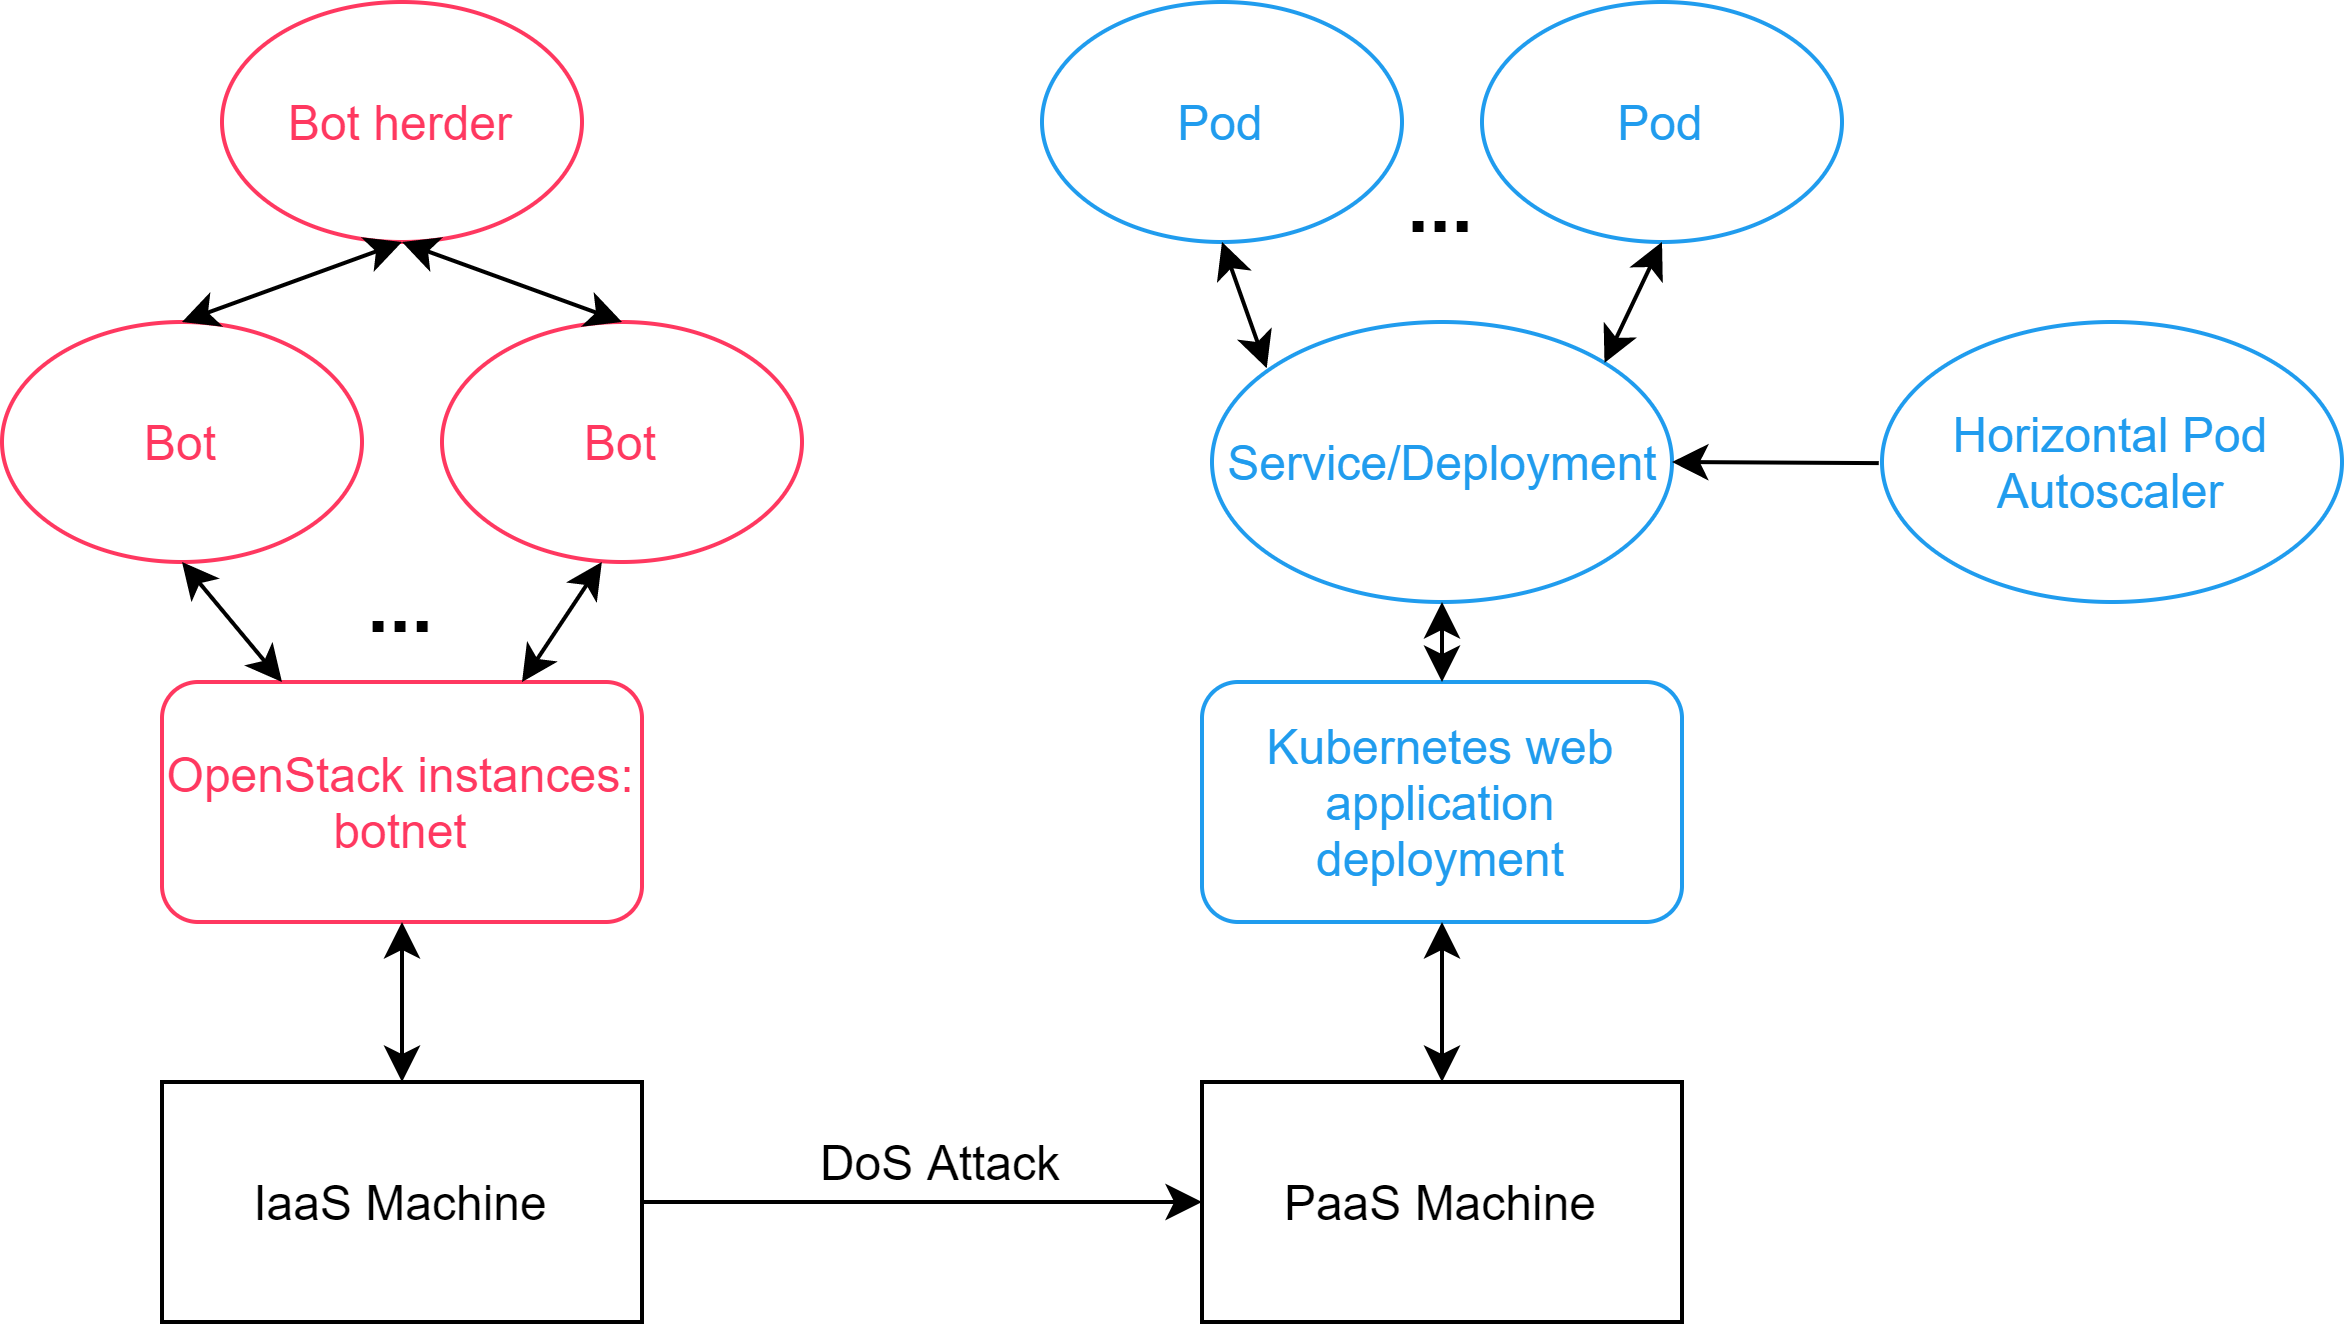
\includegraphics[scale=0.8]{schema.png}
	\captionof{figure}{Diagram of the project.}
    	\label{fig:schema}
\end{center}

\section{Infrastructure as a Service}
\label{iaas}
We will create an OpenStack project with multiple instances and a shared network that will be deployed using Terraform. The botnet will use a centralized architecture. So, one of these instances will be the "bot herder" that sends commands to the other instances. The "compromised" machines will run a simple application that allows them to receive instructions and start a DoS against a specified address (the one running in the PaaS infrastructure). Hence, each bot has to be able to reach the web application inside the PaaS machine. To sum up, for the OpenStack part we will touch project, user, images and flavors. After that, we will have to run instances that represent our bots and set up the routes in order to reach the PaaS machine.

\section{Platform as a Service}
\label{paas}
On the PaaS Infrastructure, we will run a simple web application running in a Kubernetes Pod that will be reachable from the outside network using Services. This pod will be created using a Deployment.  Then, we plan to use the Horizontal Pod Autoscaler to replicate the pod based on the load on the server (for example CPU utilization). It would also be nice to show the effects of the DoS with Autoscaler disabled or enabled and the load-balancing done by Kubernetes. So, the simple web application will be composed by at least two Docker containers: for example one may represent the backend and the other the frontend. Even for the PaaS part the entire infrastructure will be deployed using Terraform.

\section{Feasibility details}
\label{feasibility}
It will be fundamental to fine-tune both the size of the botnet and the size of the server running on Kubernetes, to not overload the two laboratory's VMs. To create the botnet, we do not know if it will be feasible to create multiple "Compromised" instances on OpenStack or if it is better to create just one instance that inside runs multiple Docker containers. Also, we do not know if the increase of CPU power used by the web server will be considerable. And if not, which is the best metric to keep track of it. In conclusion, our doubts regard on how represent the botnet and which metric considers to track the DoS attack.

\end{document}
